\chapter*{Копии экранов моделирования исходного проекта VINC (измененная программа)}
\addcontentsline{toc}{chapter}{Копии экранов моделирования исходного проекта VINC(измененная программа)}

В соответствии с вариантом 16 необходимо было изменить код проекта. Реализовать функцию по формуле (\ref{eq:D}):

\begin{equation}
	\label{eq:D}
	R[i] = A[i]*4 - 16
\end{equation}

На рисунке \ref{png:adder_func} приведен код измененнной программы.

\begin{figure}[H]
	\captionsetup{justification=centering}
	\centering{
		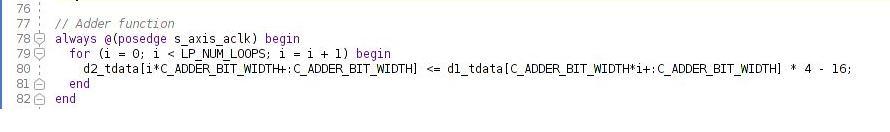
\includegraphics[scale=0.9]{images/code_2}
		\caption{Измененный код модуля \_adder.v}
		\label{png:adder_func}
	}
\end{figure}

На рисунке \ref{png:read_data_2} приведена транзакция чтения данных вектора на шине AXI4 MM из DDR памяти.
\begin{figure}[H]
	\captionsetup{justification=centering}
	\centering{
		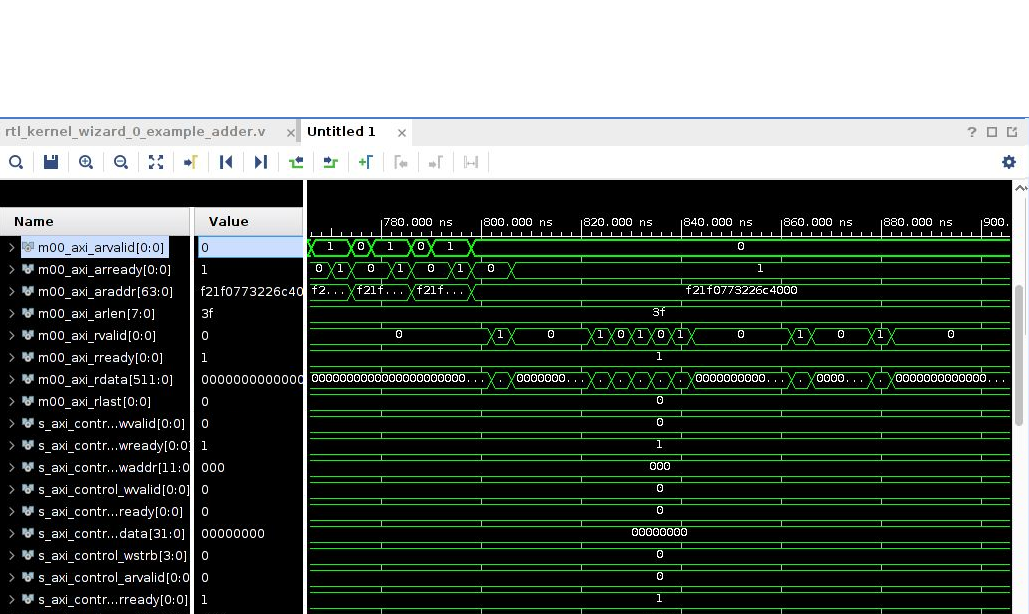
\includegraphics[scale=0.7]{images/diagram_ar_r_2}
		\caption{Транзакция чтения данных вектора на шине AXI4 MM из DDR памяти}
		\label{png:read_data_2}
	}
\end{figure}

На рисунке \ref{png:write_data_2} приведена транзакция записи результата инкремента данных на шине AXI4 MM.
\begin{figure}[H]
	\captionsetup{justification=centering}
	\centering{
		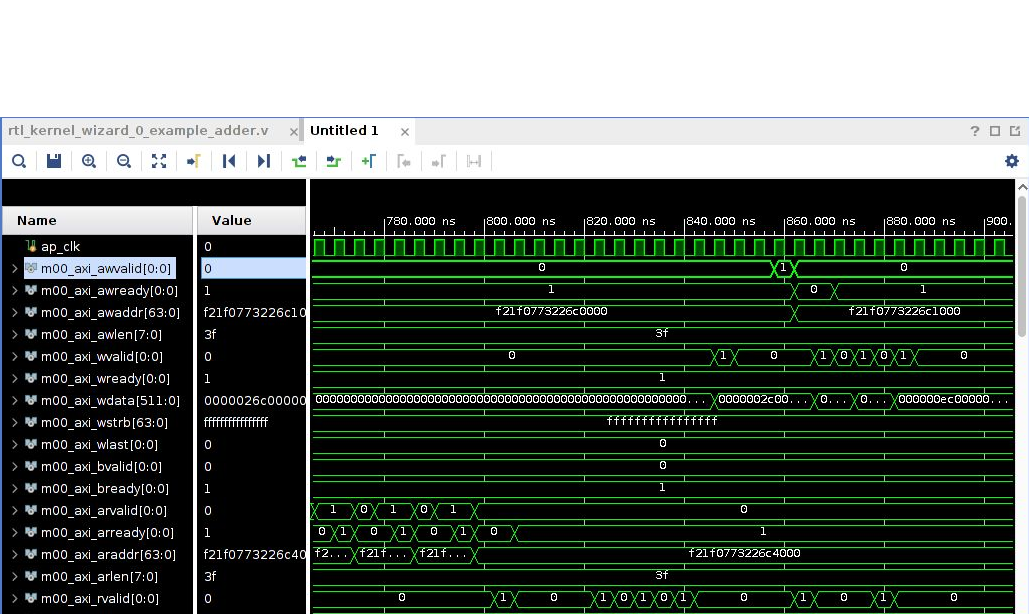
\includegraphics[scale=0.7]{images/diagram_aw_w_2}
		\caption{Транзакция записи результата инкремента данных на шине AXI4 MM}
		\label{png:write_data_2}
	}
\end{figure}